\documentclass{exam}
\usepackage{graphicx}
\usepackage[utf8]{inputenc}
\usepackage[english]{babel}
\usepackage{amsmath}
\usepackage{hyperref}
\usepackage{amsthm}
\usepackage{tcolorbox}
\usepackage{amsfonts}
\usepackage{amssymb}
\usepackage{mathrsfs}

\DeclareMathOperator{\lcm}{lcm}

\newbox\eeveebox
\setbox\eeveebox\hbox{
\raisebox{-2.5pt}{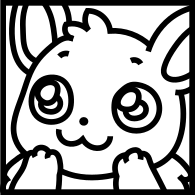
\includegraphics[height=2.5ex]{iibui.png}}}
\def\eeveeKawaii{\copy\eeveebox}

\newbox\skullbox
\setbox\skullbox\hbox{
\raisebox{-2.5pt}{
\includegraphics[height=2.5ex]{skull.png}}}
\def\bendingskull{\copy\skullbox}

\NewTColorBox{proposition}{m}{
  standard jigsaw,
  sharp corners,
  boxrule=0.4pt,
  coltitle=black,
  colframe=black,
  opacityback=0,
  opacitybacktitle=0,
  fonttitle=\normalfont\bfseries\upshape,
  fontupper=\normalfont\itshape,
  title={Proposition #1},
  after title={.},
  attach title to upper={\ },
}

\NewTColorBox{lemma}{m}{
  standard jigsaw,
  sharp corners,
  boxrule=0.4pt,
  coltitle=black,
  colframe=black,
  opacityback=0,
  opacitybacktitle=0,
  fonttitle=\normalfont\bfseries\upshape,
  fontupper=\normalfont\itshape,
  title={Lemma #1},
  after title={.},
  attach title to upper={\ },
}

\renewcommand\qedsymbol{$\eeveeKawaii$}

\title{Hammack Exercises - Chapter 8}
\author{FungusDesu}
\date{September 16th 2024}

\begin{document}

\maketitle

\section{Preface}
i dont really have anything to say

\section{Proofs Involving Sets}

\begin{proposition}{8.1}
    $\{12n:n\in\mathbb Z\}\subseteq\{2n:n\in\mathbb Z\} \cap \{3n:n\in\mathbb Z\}$.
\end{proposition}

\begin{proof}
    Suppose $a\in\{12n:n\in\mathbb Z\}$. Then $a = 12n$ for some $n\in\mathbb Z$. Consequently, $a=2\cdot(6n)$ implies $a\in\{2n:n\in\mathbb Z\}$, and $a = 3\cdot(4n)$ implies $a\in\{3n:n\in\mathbb Z\}$. Thus $a\in\{2n:n\in\mathbb Z\} \cap \{3n:n\in\mathbb Z\}$. This completes the proof.
\end{proof}

\begin{proposition}{8.2}
    $\{6n:n\in\mathbb Z\}=\{2n:n\in\mathbb Z\} \cap \{3n:n\in\mathbb Z\}$.
\end{proposition}

\begin{proof}
    $(\subseteq)$ Suppose $a\in\{6n:n\in\mathbb Z\}$. Then $a = 6n$ for some $n\in\mathbb Z$. Thus $a = 2\cdot(3n)$ implies $a\in\{2n:n\in\mathbb Z\}$, and $a=3\cdot(2n)$ implies $a\in\{3n:n\in\mathbb Z\}$. Thus $a\in\{2n:n\in\mathbb Z\}\cap\{3n:n\in\mathbb Z\}$.

    $(\supseteq)$ Suppose $a\in\{2n:n\in\mathbb Z\}\cap\{3n:n\in\mathbb Z\}$. Then $a = 2x = 3y$ for some $x,y\in\mathbb Z$. $2x$ is even, thus $3y$ must also be even implies $y$ is even. We have $y = 2k$ for some integer $k$, thus $a = 3y = 6k$. So $a$ is a multiple of 6; as such, we get $a\in\{6n:n\in\mathbb Z\}$. This completes the proof.
\end{proof}

\begin{proposition}{8.3}
    If $k\in\mathbb Z$, then $\{n\in\mathbb Z:n\mid k\}\subseteq\{n\in\mathbb Z: n\mid k^2\}$.
\end{proposition}

\begin{proof}
    Suppose $a\in\{n\in\mathbb Z: n\mid k\}$. Then $a\mid k$ implies $k = ax$ for some $x\in\mathbb Z$. Thus $k^2 = a\cdot ax^2$; so $a\mid k^2$. Therefore $a\in\{n\in\mathbb Z: n\mid k^2\}$.
\end{proof}

\begin{proposition}{8.4}
    If $m,n\in\mathbb Z$, then $\{x\in\mathbb Z:mn\mid x\}\subseteq \{x\in\mathbb Z:m\mid x\}\cap\{x\in\mathbb Z: n\mid x\}$.
\end{proposition}

\begin{proof}
    Suppose $a\in\{x\in\mathbb Z:mn\mid x\}$. Then $mn\mid a$ implies $a=mnk$ for some integer $k$. Thus $a = m\cdot(nk) = n\cdot(mk)$ implies $m \mid a$ and $n\mid a$. Therefore $a\in\{x\in\mathbb Z:m\mid x\}$ and $a\in\{x\in\mathbb Z: n\mid x\}$; and so $a\in\{x\in\mathbb Z:m\mid x\}\cap\{x\in\mathbb Z: n\mid x\}$.
\end{proof}

\begin{proposition}{8.5}
    If $p$ and $q$ are positive integers, then $\{pn:n\in\mathbb N\}\cap\{qn:n\in\mathbb N\}\neq\varnothing$.
\end{proposition}

\begin{proof}
    Note that $pq$ is both a element of $\{pn:n\in\mathbb N\}$ and $\{qn:n\in\mathbb N\}$. Thus $\{pn:n\in\mathbb N\}\cap\{qn:n\in\mathbb N\}$ always has at least one element, namely $pq$.
\end{proof}

\begin{proposition}{8.6}
    Suppose $A,B$ and $C$ are sets. If $A\subseteq B$, then $A-C\subseteq B-C$.
\end{proposition}

\begin{proof}
    Suppose $a\in A - C$. Then $a\in A$ and $a\notin C$. But because $A\subseteq B$, we have $a\in B$ and $a\notin C$. Thus $a\in B - C$. And so $A - C \subseteq B - C$, as desired.
\end{proof}

\begin{proposition}{8.7}
    Suppose $A, B$ and $C$ are sets. If $B\subseteq C$, then $A\times B\subseteq A\times C$.
\end{proposition}

\begin{proof}
    Let $a\in A$ and $b\in B$. Then we have $(a, b)\in A\times B$. Since $B\subseteq C$, we have $b\in B$ implies $b\in C$. Thus it is also true that $(a, b)\in A\times C$. Therefore $(a, b) \in A\times B$ implies $(a, b)\in A \times C$, and so $A\times B \subseteq A\times C$.
\end{proof}

\begin{proposition}{8.8}
    If $A, B$ and $C$ are sets, then $A\cup(B\cap C)=(A\cup B)\cap(A\cup C)$.
\end{proposition}

\begin{proof}
    Observe that:
    \begin{align*}
        A\cup (B\cap C) &= \{x:x\in A \lor x \in B\cap C\}\\
        &=\{x:x\in A\lor(x\in B \land x\in C)\}\\
        &=\{x:(x\in A\lor x\in B) \land (x\in A \lor x \in C)\}.
    \end{align*}
    We can confirm the previous line is indeed true by the following truth table:
    \begin{center}
        \begin{tabular}{|c|c|c||c||c|}
            \hline
            $x\in A$ & $x\in B$ & $x\in C$ & $x\in A\lor(x\in B\land x\in C)$ & $(x\in A\lor x\in B)\land(x\in A\lor x\in C)$\\
            \hline\hline
            T&T&T&T&T\\
            \hline
            T&T&F&T&T\\
            \hline
            T&F&T&T&T\\
            \hline
            T&F&F&T&T\\
            \hline
            F&T&T&T&T\\
            \hline
            F&T&F&F&F\\
            \hline
            F&F&T&F&F\\
            \hline
            F&F&F&F&F\\
            \hline
        \end{tabular}
    \end{center}
    Thus, it follows that:
    \begin{align*}
        A\cup (B\cap C) &=\{x:(x\in A\lor x\in B) \land (x\in A \lor x \in C)\}\\
        &=\{x:(x\in A\lor x\in B)\}\cap\{x:(x\in A\lor x\in c)\}\\
        &=(A\cup B)\cap(A\cup C).
    \end{align*}
    This completes our proof.
\end{proof}

\begin{proposition}{8.9}
    If $A,B$ and $C$ are sets, then $A\cap (B\cup C)=(A\cap B)\cup(A\cap C)$.
\end{proposition}

\begin{proof}
    Observe that:
    \begin{align*}
        A\cap(B\cup C) &= \{x:x\in A\land(x\in B\lor x\in C)\}\\
        &= \{x: (x\in A\land x\in B)\lor(x\in A\land x\in C)\}.
    \end{align*}
    The following truth table justifies this equality:
    \begin{center}
        \begin{tabular}{|c|c|c||c||c|}
            \hline
            $x\in A$ & $x\in B$ & $x\in C$ & $x\in A\land(x\in B\lor x\in C)$ & $(x\in A\land x\in B)\lor(x\in A\land x\in C)$\\
            \hline\hline
            T&T&T&T&T\\
            \hline
            T&T&F&T&T\\
            \hline
            T&F&T&T&T\\
            \hline
            T&F&F&F&F\\
            \hline
            F&T&T&F&F\\
            \hline
            F&T&F&F&F\\
            \hline
            F&F&T&F&F\\
            \hline
            F&F&F&F&F\\
            \hline
        \end{tabular}
    \end{center}
    Thus, it follows that:
    \begin{align*}
        A\cap(B\cup C) &= \{x: (x\in A\land x\in B)\lor(x\in A\land x\in C)\}\\
        &= (A\cap B)\cup(A\cap C).
    \end{align*}
    This completes our proof.
\end{proof}

\begin{proposition}{8.10}
    If $A$ and $B$ are sets in a universal set $U$, then $\overline{A\cap B}=\overline A\cup\overline B$.
\end{proposition}

\begin{proof}
    Simply observe the following chain of equalities:
    \begin{align*}
        \overline{A\cap B}&=\{x:\lnot(x\in A\land x\in B)\}\\
        &=\{x:\lnot(x\in A)\lor\lnot(x\in B)\}\\
        &=\overline A\cup\overline B.
    \end{align*}
\end{proof}

\begin{proposition}{8.11}
    If $A$ and $B$ are sets in a universal set $U$, then $\overline{A\cup B}=\overline A\cap\overline B$.
\end{proposition}

\begin{proof}
    Simply observe the following chain of equalities:
    \begin{align*}
        \overline{A\cup B}&=\{x:\lnot(x\in A\lor x\in B)\}\\
        &=\{x:\lnot(x\in A)\land\lnot(x\in B)\}\\
        &=\overline A\cap\overline B.
    \end{align*}
\end{proof}

\begin{proposition}{8.12}
    If $A, B$ and $C$ are sets, then $A-(B\cap C)=(A-B)\cup(A-C)$
\end{proposition}

\begin{proof}
    Simply observe the following chain of equalities:
    \begin{align*}
        A-(B\cap C)&=\{x:x\in A\land(\lnot(x\in B\land x\in C))\}\\
        &=\{x:x\in A\land(\lnot(x\in B)\lor\lnot(x\in C))\}\\
        &=\{x:(x\in A\land\lnot(x\in B))\lor(x\in A\land\lnot(x\in C))\}\\
        &=\{x:x\in(A - B)\lor x\in(A- C)\}\\
        &= (A-B)\cup(A-C).
    \end{align*}
\end{proof}

\begin{proposition}{8.13}
    If $A, B$ and $C$ are sets, then $A-(B\cup C)=(A-B)\cap(A-C)$
\end{proposition}

\begin{proof}
    Simply observe the following chain of equalities:
    \begin{align*}
        A-(B\cup C)&=\{x:x\in A\land(\lnot(x\in B\lor x\in C))\}\\
        &=\{x:x\in A\land x\in A\land\lnot(x\in B)\land\lnot(x\in C)\}\\
        &=\{x:(x\in A\land\lnot(x\in B))\land(x\in A\land\lnot(x\in C))\}\\
        &=\{x:x\in(A - B)\land x\in(A- C)\}\\
        &= (A-B)\cap(A-C).
    \end{align*}
\end{proof}

\begin{proposition}{8.14}
    If $A, B$ and $C$ are sets, then $(A\cup B) - C = (A - C)\cup(B - C)$.
\end{proposition}

\begin{proof}
    Simply observe the following chain of equalities:
    \begin{align*}
        (A\cup B)-C &= \{x: (x\in A\lor x\in B)\land\lnot(x\in C)\}\\
        &= \{x:(x\in A\land\lnot(x\in C))\lor(x\in B\land\lnot(x\in C))\}\\
        &= \{x:(x\in A - C)\lor(x\in B - C)\}\\
        &= (A-C)\cup(B-C).
    \end{align*}
\end{proof}

\begin{proposition}{8.15}
    If $A, B$ and $C$ are sets, then $(A\cap B) - C = (A - C)\cap(B - C)$.
\end{proposition}

\begin{proof}
    Simply observe the following chain of equalities:
    \begin{align*}
        (A\cap B)-C &= \{x: x\in A\land x\in B\land\lnot(x\in C)\}\\
        &= \{x:(x\in A\land\lnot(x\in C))\land(x\in B\land\lnot(x\in C))\}\\
        &= \{x:(x\in A - C)\land(x\in B - C)\}\\
        &= (A-C)\cap(B-C).
    \end{align*}
\end{proof}

\begin{proposition}{8.16}
    If $A, B$ and $C$ are sets, then $A\times (B\cup C)=(A\times B)\cup (A\times C)$.
\end{proposition}

\begin{proof}
    Simply observe the following chain of equalities:
    \begin{align*}
        A\times(B\cup C) &=\{(x, y): x\in A\land (y\in B\lor y\in C)\}\\
        &=\{(x, y):(x\in A\land y\in B) \lor(x\in A\land y\in C)\}\\
        &=\{(x, y):x\in A\land y\in B\}\cup\{(x, y):x\in A\land y\in C\}\\
        &=(A\times B)\cup(A\times C).
    \end{align*}
\end{proof}

\begin{proposition}{8.17}
    If $A, B$ and $C$ are sets, then $A\times (B\cap C)=(A\times B)\cap (A\times C)$.
\end{proposition}

\begin{proof}
    This is proven in Example 8.13.
\end{proof}

\begin{proposition}{8.18}
    If $A, B$ and $C$ are sets, then $A\times(B-C)=(A\times B)-(A\times C)$.
\end{proposition}

\begin{proof}
    Simply observe the following chain of equalities:
    \begin{align*}
        A\times(B-C)&=\{(x, y): x\in A\land y\in B\land \lnot(y\in C)\}\\
        &=\{(x, y):(x\in A\land y\in B)\land\lnot(x\in A\land y\in C)\}.
    \end{align*}
    This can be justified by the following truth table:
    \begin{center}
        \begin{tabular}{|c|c|c||c||c|}
            \hline
            $x\in A$ & $y\in B$ & $y\in C$ & $x\in A\land y\in B\land \lnot(y\in C)$ & $(x\in A\land y\in B)\land\lnot(x\in A\land y\in C)$\\
            \hline\hline
            T&T&T&F&F\\
            \hline
            T&T&F&T&T\\
            \hline
            T&F&T&F&F\\
            \hline
            T&F&F&F&F\\
            \hline
            F&T&T&F&F\\
            \hline
            F&T&F&F&F\\
            \hline
            F&F&T&F&F\\
            \hline
            F&F&F&F&F\\
            \hline
        \end{tabular}
    \end{center}
    Thus, it follows that
    \begin{align*}
        A\times(B-C)&=\{(x, y):(x\in A\land y\in B)\land\lnot(x\in A\land y\in C)\}\\
        &=\{(x, y):x\in A\land y\in B\}\cap\{(x, y): x\notin A\lor y\notin C\}\\
        &=\{(x, y):(x, y)\in(A\times B)\}\cap\{(x, y): (x,y)\notin(A\times C)\}\\
        &=(A\times B)-(A\times C).
    \end{align*}
    This completes our proof.
\end{proof}

\begin{proposition}{8.19}
    $\{9^n:n\in\mathbb Z\}\subseteq\{3^n: n\in\mathbb Z\}$, but $\{9^n:n\in\mathbb Z\}\neq \{3^n:n\in\mathbb Z\}$.
\end{proposition}

\begin{proof}
    Let $a\in\{9^n:n\in\mathbb Z\}$. Then $a = 9^n$ for some integer $n$. Note that $a = 9^n = 3^{2n}$. Thus $a\in\{3^n:n\in\mathbb Z\}$, and consequently $\{9^n:n\in\mathbb Z\}\subseteq\{3^n: n\in\mathbb Z\}$. Notice that $3$ is an element of $\{3^n:n\in\mathbb Z\}$. Since there does not exist $x\in\mathbb Z$ such that $9^x = 3$, we know $3\notin\{9^n:n\in\mathbb Z\}$. Thus $\{9^n:n\in\mathbb Z\}\neq \{3^n:n\in\mathbb Z\}$, and we are done.
\end{proof}

\begin{proposition}{8.20}
    $\{9^n:n\in\mathbb Q\}=\{3^n:n\in\mathbb Q\}$.
\end{proposition}

\begin{proof}
    $(\subseteq)$ Suppose $x\in\{9^n:n\in\mathbb Q\}$. Then $x = 9^n$ for some rational $n$. Note that $x= 9^n = 3^{2n}$, and so $x\in\{3^n:n\in\mathbb Q\}$.

    $(\supseteq)$ Suppose $x\in\{3^n:n\in\mathbb Q\}$. Then $x=3^n$ for some rational $n$. Note that $x = 3^n = 9^{\frac n 2}$, and so $x\in\{9^n:n\in\mathbb Q\}$. This completes our proof.
\end{proof}

\begin{proposition}{8.21}
    Suppose $A$ and $B$ are sets. $A\subseteq B$ if and only if $A - B=\varnothing$.
\end{proposition}

\begin{proof}
    $(\implies)$ Suppose to the contrary that there exists $x\in A - B$. Then $x\in A$ and $x\notin B$. But we also have $A\subseteq B$, which contradicts this fact.

    $(\impliedby)$ Suppose to the contrary that $A\nsubseteq B$. Then there exists $x\in A$ and $x\notin B$. But this contradicts the fact that $A-B=\varnothing$. This completes our proof.
\end{proof}

\begin{proposition}{8.22}
    Let $A$ and $B$ be sets. $A\subseteq B$ if and only if $A\cap B=A$.
\end{proposition}

\begin{proof}
    $(\implies)$ Suppose to the contrary that $A\cap B\neq A$. Then there exists $x\in A$ and $x\notin B$. But this contradicts the fact that $A\subseteq B$.

    $(\impliedby)$ Suppose to the contrary that $A\nsubseteq B$. Then there exists $x\in A$ and $x\notin B$. But this contradicts the fact that $A\cap B = A$. This completes our proof.
\end{proof}

\begin{proposition}{8.23}
    For each $a\in\mathbb R$, let $A_a=\{(x,a(x^2-1))\in\mathbb R^2:x\in\mathbb R\}$. Then $$\bigcap_{a\in\mathbb R}A_a=\{(-1, 0), (1, 0)\}.$$
\end{proposition}

\begin{proof}
    Note that $A_a=\{(x,a(x^2-1))\in\mathbb R^2:x\in\mathbb R\}$ represents the graph of $y=a(x^2-1)$ for some real $a$; and so $\bigcap_{a\in\mathbb R}A_a$ represents the set of points that $A_a$ always passes through for all real $a$. We shall first show that $\{(-1, 0), (1, 0)\}$ are two members of $\bigcap_{a\in\mathbb R}A_a$.

    $(\supseteq)$ Suppose $(x,y)\in\{(-1, 0), (1, 0)\}$. Then for all real $a$, we can see that $(x,y)\in A_a$ ($0=a((-1)^2-1)=0,0=a((1)^2-1)=0$). Thus 
    \[
    (x, y)\in\bigcap_{a\in\mathbb R}A_a.
    \]

    $(\subseteq)$ Suppose $(x,y)\in\bigcap_{a\in\mathbb R}A_a$. Consider $A_{420}\cap A_{0.69}$. This represents the set of common points of $y=420(x^2-1)$ and $y=0.69(x^2-1)$; in other words, the roots of $420(x^2-1)=0.69(x^2-1)$. Thus:
    \begin{align*}
        420(x^2-1)=0.69(x^2-1)\iff419.31x^2=419.31\iff x^2&=1\iff x=1\lor x=-1
    \end{align*}
    At $x=1$ or $x=-1$, we have $y=0$. Thus $(x,y)\in\{(-1,0),(1,0)\}$. This completes our proof.
\end{proof}

\begin{proposition}{8.24}
    $$\bigcap_{x\in\mathbb R}[3-x^2,5+x^2]=[3, 5].$$
\end{proposition}

\begin{proof}
    $(\supseteq)$ Suppose $a\in[3,5]$. For all real $x$, we have $3-x^2 \le 3$ and $5+x^2\ge 5$. Thus $[3, 5]\subseteq[3-x^2, 5+x^2]$ for all real $x$. Therefore \[
    a\in\bigcap_{x\in\mathbb R}[3-x^2,5+x^2].
    \]

    $(\subseteq)$ Suppose $a\in\bigcap_{x\in\mathbb R}[3-x^2,5+x^2]$. Let $\bendingskull_x=[3-x^2,5+x^2]$; consider $\bendingskull_0$. Then $\bendingskull_0 = [3-0^2, 5+0^2]=[3, 5]\subseteq [3,5]$. Thus $a\in[3, 5]$. This completes our proof.
\end{proof}

\begin{proposition}{8.25}
    Suppose $A, B, C$ and $D$ are sets. Then $(A\times B)\cup(C\times D)\subseteq(A\cup C)\times (B\cup D)$.
\end{proposition}

\begin{proof}
    Suppose $(x,y)\in(A\times B)\cup(C\times D)$. Then we have the following:
    \begin{align*}
        (x,y)\in(A\times B)\cup(C\times D)&\implies(x, y)\in(A\times B)\lor(x, y)\in(C\times D)\\
        &\implies(x\in A\land y\in B)\lor(x\in C\land y\in D)\\
        &\implies(x\in A\lor x\in C)\land(y\in B\lor y\in D)\\
        &\implies x\in A\cup C\land y\in B\cup D\\
        &\implies (x, y)\in(A\cup C)\times(B\cup D),
    \end{align*}
    and we are done.
\end{proof}

\begin{proposition}{8.26}
    $\{4k + 5:k\in\mathbb Z\}=\{4k+1:k\in\mathbb Z\}$.
\end{proposition}

\begin{proof}
    $(\subseteq)$ Suppose $\bendingskull\in\{4k + 5:k\in\mathbb Z\}$. Thus $\bendingskull = 4k+5$ for some integer $k$. Note that $\bendingskull = 4k + 5 = 4(k+1)+1$, thus $\bendingskull\in\{4k + 1:k\in\mathbb Z\}$.

    $(\supseteq)$ Suppose $\bendingskull\in\{4k+1:k\in\mathbb Z\}$. Thus $\bendingskull=4k +1$ for some integer $k$. Note that $\bendingskull=4k+1 =4(k-1)+5$, thus $\bendingskull\in\{4k + 5:k\in\mathbb Z\}$. This completes our proof.
\end{proof}

\begin{proposition}{8.27}
    $\{12a+4b:a, b\in\mathbb Z\}=\{4c:c\in\mathbb Z\}$.
\end{proposition}

\begin{proof}
    $(\subseteq)$ Suppose $x\in\{12a+4b:a, b\in\mathbb Z\}$. Then $x=12a + 4b$ for some integer $a, b$. Note that $x = 12a + 4b = 4(3a + b)$. Thus $x\in\{4c:c\in\mathbb Z\}$.

    $(\supseteq)$ Suppose $x\in\{4c: c\in\mathbb Z\}$. Then $x = 4c$ for some integer $c$. Note that $x = 4c = 12\cdot 0 + 4c$. Thus $x\in\{12a + 4b: a,b\in\mathbb Z\}$, and we are done.
\end{proof}

\begin{proposition}{8.28}
    $\{12a + 25b:a,b\in\mathbb Z\}=\mathbb Z$.
\end{proposition}

\begin{proof}
    $(\subseteq)$. Suppose $k\in\{12a+25b:a,b\in\mathbb Z\}$. Thus $k=12a+25b$ for some integer $a, b$. Therefore $k\in\mathbb Z$.

    $(\supseteq)$. Suppose $k\in\mathbb Z$. Note that there exist $x,y$ such that $12x + 25y=\gcd(12, 25) = 1$ by Proposition 7.1. Thus we have $12xk + 25yk = k$. Thus $k\in\{12a + 25b:a,b\in\mathbb Z\}$. This completes our proof.
\end{proof}

\begin{proposition}{8.29}
    Suppose $A\neq\varnothing$. Then $A\times B\subseteq A\times C$ if and only if $B\subseteq C$.
\end{proposition}

\begin{proof}
    $(\implies)$ Suppose $x\in B$. Because $A\neq\varnothing$, there exists $a\in A$. Thus $(a, x)\in(A\times B)$. But because $A\times B\subseteq A\times C$, we have $(a, x)\in(A\times C)$. Thus $x\in C$. Therefore $B\subseteq C$.

    $(\impliedby)$ Suppose $(x, y)\in(A\times B)$; thus $x\in A$ and $y\in B$. Since $B\subseteq C$, we have $y\in C$, and so $(x, y)\in (A\times C)$. Therefore $A\times B\subseteq A\times C$, and we are done.
\end{proof}

\begin{lemma}{8.1}
    Suppose $A, B, C$ and $D$ are sets. Then $(A\times B)\cap(C\times D)=(A\cap C)\times(B\cap D)$.
\end{lemma}

\begin{proof}
    Suppose $(x, y) \in (A\times B)\cap(C\times D)$. Then we have the following:
    \begin{align*}
        (x, y) \in (A\times B)\cap(C\times D)&\iff x\in A\land y \in B\land x\in C\land y\in D\\
        &\iff (x\in A\cap C)\cap(y\in B\cap D)\\
        &\iff (x, y)\in (A\cap C)\times(B\cap D).
    \end{align*}
\end{proof}

\begin{proposition}{8.30}
    $(\mathbb Z\times\mathbb N)\cap(\mathbb N\times \mathbb Z) = \mathbb N\times \mathbb N$.
\end{proposition}

\begin{proof}
    By Lemma 8.1, we have the following:
    \begin{align*}
        (\mathbb Z\times\mathbb N)\cap(\mathbb N\times \mathbb Z) = (\mathbb Z\cap\mathbb N)\times(\mathbb N\cap \mathbb Z) = \mathbb N\times\mathbb N.
    \end{align*}
\end{proof}

\begin{proposition}{8.31}
    Suppose $B\neq\varnothing$ and $A\times B\subseteq B\times C$. Then $A\subseteq C$.
\end{proposition}

\begin{proof}
    Suppose $x\in A$. Since $B\neq\varnothing$, there exists $y\in B$. Thus $(x, y) \in (A\times B)$; because $(A\times B)\subseteq (B\times C)$, we have $(x, y) \in (A\times C)$. Therefore $y\in C$, and we are done.
\end{proof}

\end{document}